\documentclass[oneside,a4paper,14pt]{extarticle}
\usepackage[T1,T2A,TU]{fontenc}
\usepackage[a4paper,letterpaper,top=20mm,bottom=20mm,left=20mm,right=10mm]{geometry}
\usepackage[russian]{babel}
\usepackage{textcomp}
\usepackage{indentfirst}
\usepackage{graphicx}
\usepackage{mwe}
\usepackage{wrapfig}
\usepackage{caption}
\usepackage{amsmath}
\usepackage{amsfonts}
\usepackage{amsthm}
\usepackage{amssymb}
\usepackage[all]{xy}
\usepackage[breaklinks]{hyperref}
\usepackage{titlesec}
\usepackage{verbatim, fancyvrb}
\usepackage{xcolor}

\titleformat{\section} % Настройка формата заголовков секций
{\normalsize\bfseries} % Устанавливает размер шрифта на нормальный и делает его жирным
{\thesection} % Указывает, что номер секции будет отображаться перед заголовком
{1em} % Устанавливает расстояние между номером секции и заголовком в 1em
{} % Дополнительные параметры.

\titleformat{\subsection} % Настройка формата заголовков подсекций
{\normalsize\bfseries} % Устанавливает размер шрифта на нормальный и делает его жирным
{\thesubsection} % Указывает, что номер подсекции будет отображаться перед заголовком
{1em} % Устанавливает расстояние между номером подсекции и заголовком в 1em
{} % Дополнительные параметры.

\titleformat{\subsubsection} % Настройка формата заголовков подподсекций
{\normalsize\bfseries} % Устанавливает размер шрифта на нормальный и делает его жирным
{\thesubsection} % Указывает, что номер подподсекции будет отображаться перед заголовком
{1em} % Устанавливает расстояние между номером подподсекции и заголовком в 1em
{} % Дополнительные параметры.

\renewcommand\baselinestretch{1.45}\normalsize %межстр интервал
\setlength{\parindent}{1.25cm} %длина отступа нового абзаца

\begin{document}
\newpage
\thispagestyle{empty}
\begin{center}
	МИНИСТЕРСТВО НАУКИ И ВЫСШЕГО ОБРАЗОВАНИЯ\\
	РОССИЙСКОЙ ФЕДЕРАЦИИ
	ФЕДЕРАЛЬНОЕ ГОСУДАРСТВЕННОЕ БЮДЖЕТНОЕ\\
	ОБРАЗОВАТЕЛЬНОЕ
	УЧРЕЖДЕНИЕ ВЫСШЕГО ОБРАЗОВАНИЯ\\
	«ВЯТСКИЙ ГОСУДАРСТВЕННЫЙ УНИВЕРСИТЕТ»\\
	Институт математики и информационных систем\\
	Факультет автоматики и вычислительной техники\\
	Кафедра электронных вычислительных машин
\end{center}
\vspace{20mm}

\begin{center}
	Отчёт по лабораторной работе №6\\
	по дисциплине\\
	<<Информатика>>\\
	<<Кодирование информации.>>\\
\end{center}
\vspace{40mm}
\noindent
\begin{tabular}{ll}
	Разработал студент гр. ИВТб-1301-05-00 & \rule[-1mm]{30mm}{0.10mm}\,/Черкасов А. А./ \\
	                                       & \hspace{8mm}\footnotesize(подпись)          \\

	Проверил доцент кафедры ЭВМ            & \rule[-1mm]{30mm}{0.10mm}\,/Коржавина А.С./ \\
	                                       & \hspace{8mm}\footnotesize(подпись)          \\
\end{tabular}

\vfill
\begin{center}
	Киров\\
	2024
\end{center}

\newpage\thispagestyle{plain}
\section*{Цель работы}
Цель работы: Изучить методы и алгоритмы кодирования информации. Реализовать
равномерное кодирование и оптимальное кодирование с использованием алгоритмов
Фано или Хаффмана, проанализировать их свойства и применимость в различных
задачах.

\section*{Задания}
\begin{enumerate}
	\item \textbf{Равномерное кодирование.}\\
	      Написать программу, выполняющую кодирование N различных состояний равномерно.\\
	      \textbf{Формат Ввода.} \\
	      Целое число N -- количество различных состояний. \\
	      \textbf{Формат Вывода.} \\
	      Список кодов.
	      $$
		      \begin{tabular}{ll}
			      \textbf{Ввод} & \textbf{Вывод}          \\
			      \hline
			      6             & 000 001 010 011 100 101 \\
			      \hline
		      \end{tabular}
	      $$
	\item \textbf{Оптимальное кодирование.}\\
	      Написать программу, выполняющую кодирование алгоритмом Хаффмана или Фано.\\
	      \textbf{Формат Ввода.} \\
	      Через пробел количество событий (кодовых состояний) и массив вероятностей каждого из событий. \\
	      \textbf{Формат Вывода.} \\
	      Коды состояний.
	      $$
		      \begin{tabular}{ll}
			      \textbf{Ввод}        & \textbf{Вывод} \\
			      \hline
			      4 0.5 0.25 0.13 0.12 & 0 10 110 111   \\
			      \hline
		      \end{tabular}
	      $$
\end{enumerate}
\newpage

\section*{Решение}
\noindent Схемы алгоритмов представлены на Рисунках 1.1, 1.2 и 1.3. \\
\noindent Код программ приведён в Приложениях A1 и А2.\\
\begin{figure}[h!]
	\centering
	%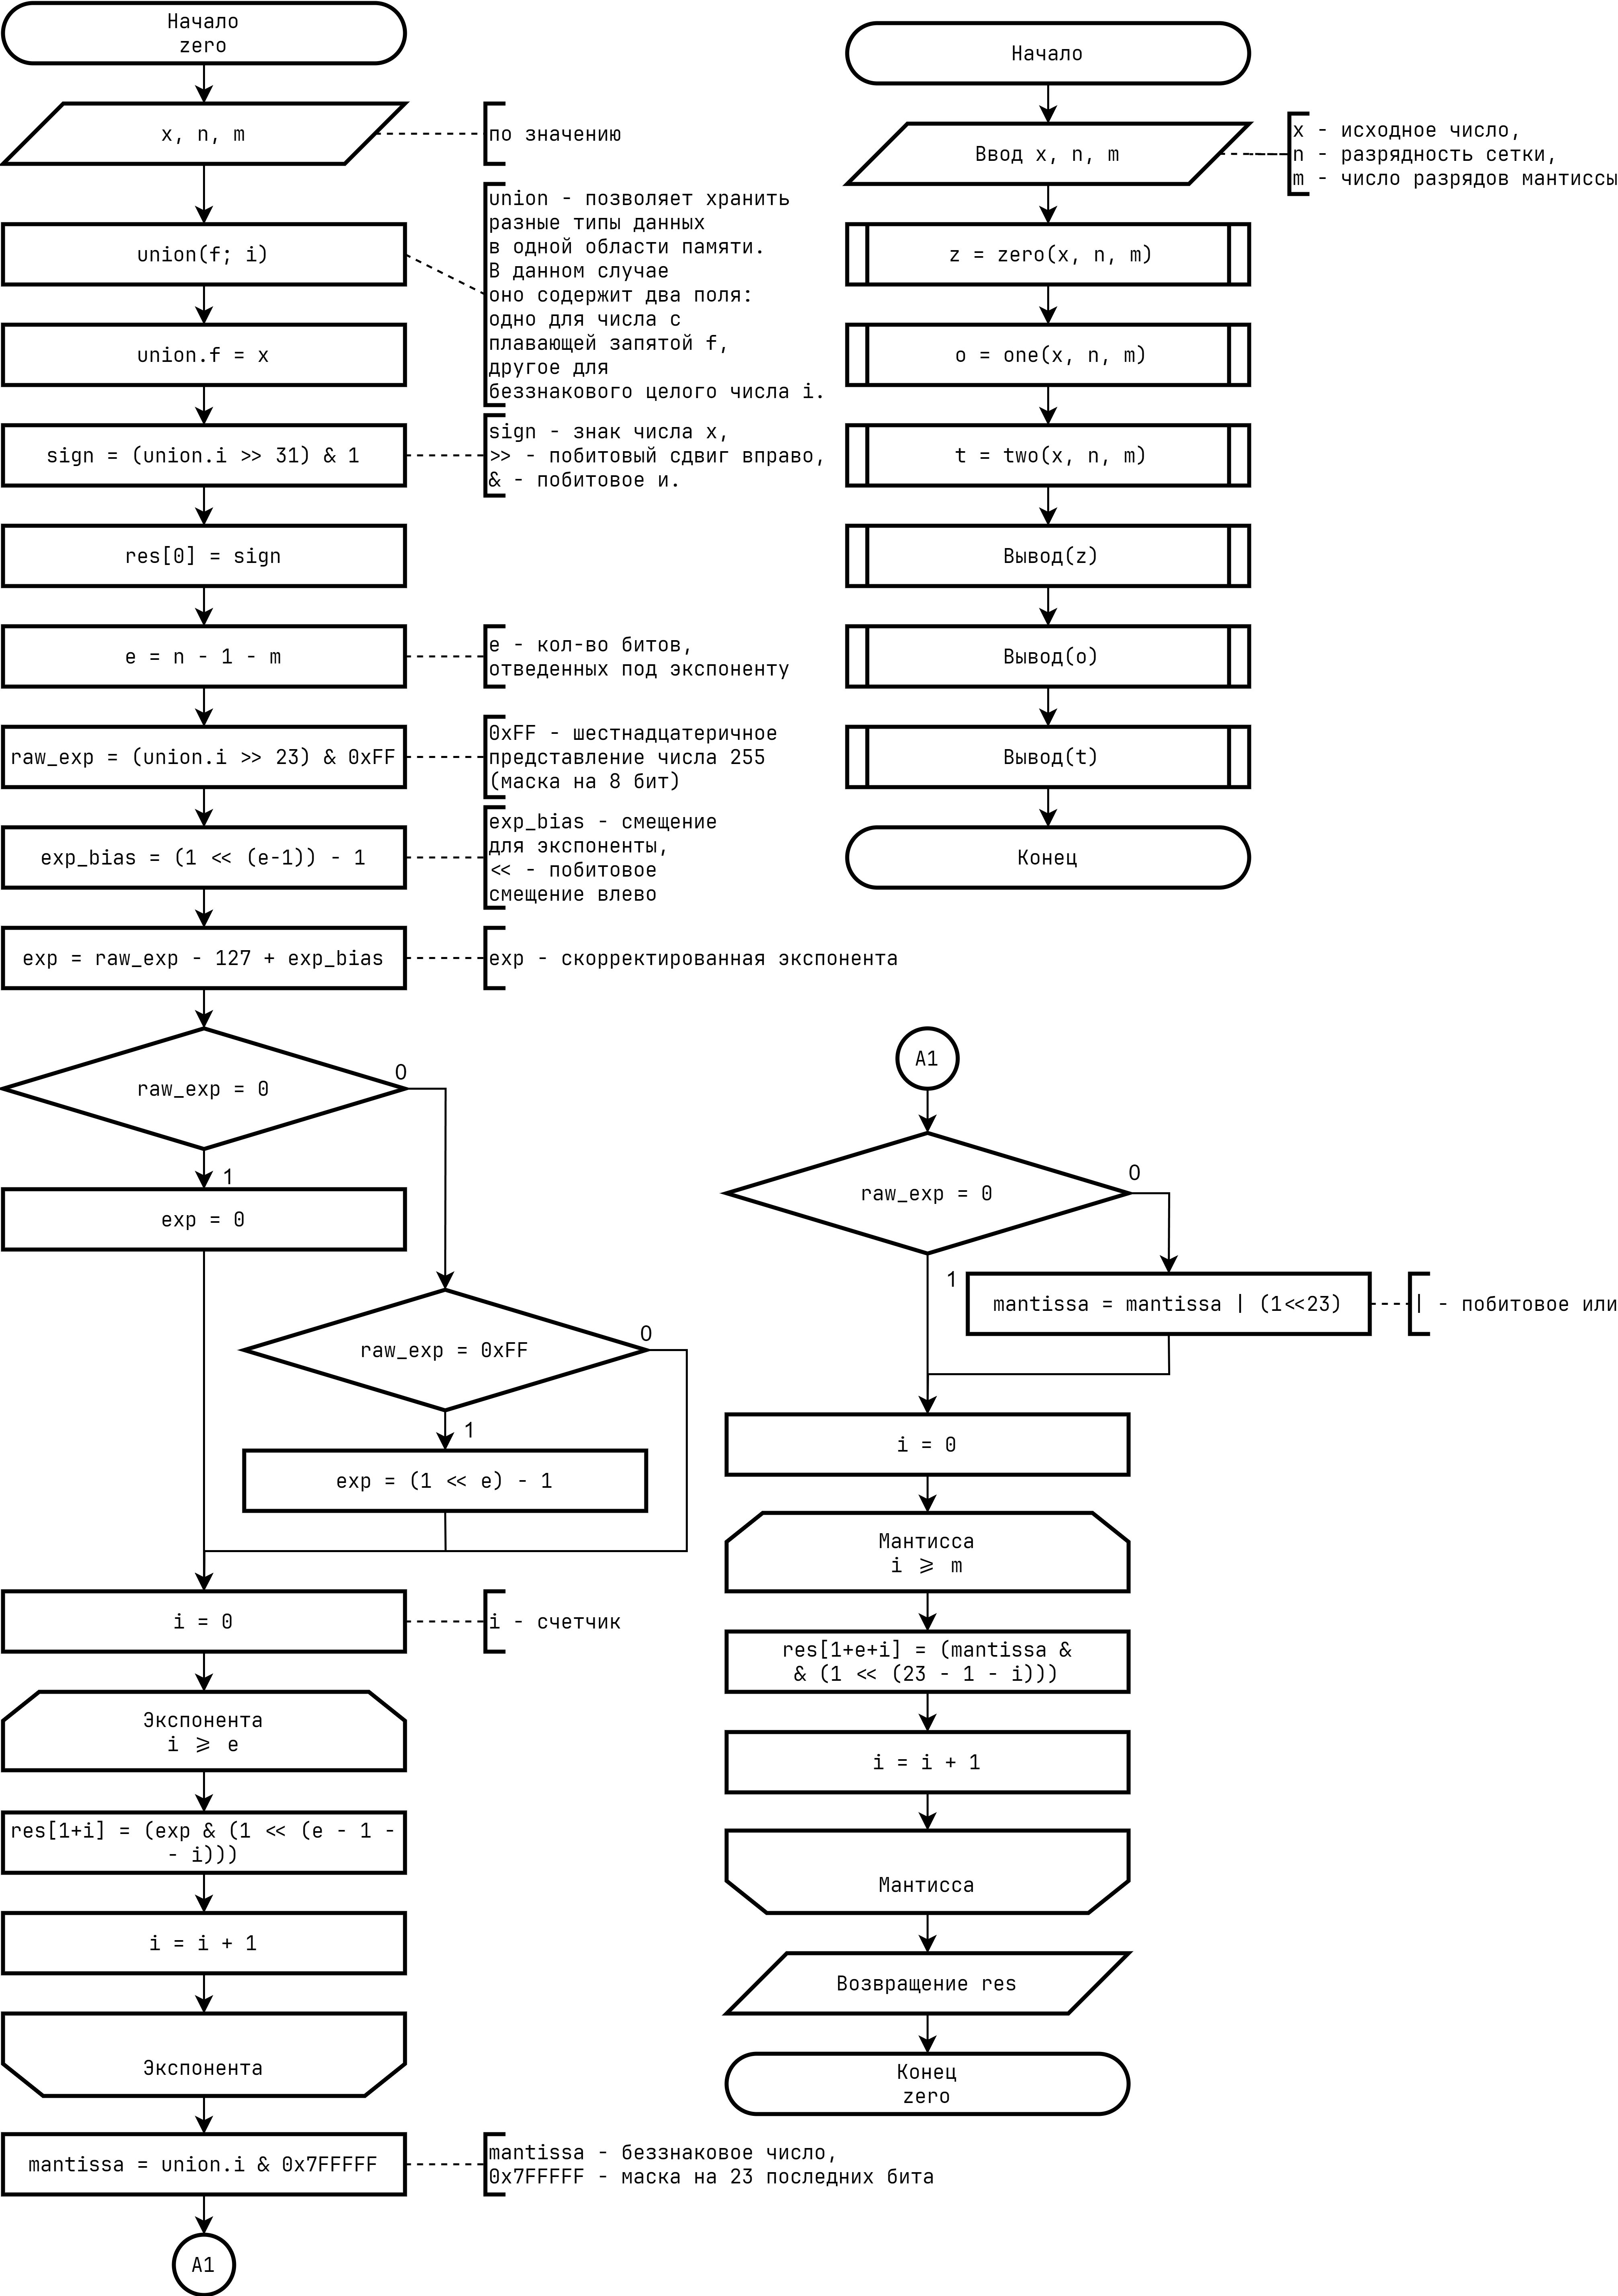
\includegraphics[height=0.75\textheight]{pics/5_flowchart_p1.png}
	\caption*{Рисунок 1.1 - Схема алгоритма программы.}
\end{figure}


\newpage
\section*{Вывод}
В результате работы разработаны программы для равномерного и оптимального
кодирования данных. Программы корректно обрабатывают входные данные и формируют
коды в соответствии с заданными алгоритмами. Тестирование подтвердило их
корректность и эффективность.\\
\newpage
\begin{flushright}
    \textcolor{black!30}{\textbf{Приложения}}
\end{flushright}
\section*{Приложение А1}
\VerbatimInput[fontsize=\small]{code/1.c}
\newpage
\section*{Приложение А2}
\VerbatimInput[fontsize=\small]{code/2.c}

\end{document}